\documentclass{article}
\usepackage{graphicx} % Required for inserting images
\usepackage{ctex}

\usepackage{amsfonts}
\usepackage{amssymb}
\usepackage{amsmath}
\usepackage{amsthm}
% 导入 xparse 宏包以支持 LaTeX3 语法
\usepackage{xparse}
\usepackage{pgfplots}
% 用于插入带有坐标轴、标签和曲线的图像

% \begin{tikzpicture}
%     \begin{axis}[
%       xlabel=$x$,
%       ylabel=$f(x)$,
%       axis lines=middle,
%       xmin=-5, xmax=5,
%       ymin=-2, ymax=8,
%       width=\textwidth,
%       height=8cm
%     ]
%     \addplot[blue,domain=-3:3] {x^2};
%     \end{axis}
%   \end{tikzpicture}
\usepackage{tikz}
% 用于绘制一般的图像

% \begin{tikzpicture}[scale=0.8]
%     \draw[->] (-4,0) -- (4,0) node[right] {$x$};
%     \draw[->] (0,-1) -- (0,9) node[above] {$f(x)$};
%     \draw[domain=-3:3,smooth,variable=\x,blue] plot ({\x},{\x^2});
%   \end{tikzpicture}

\newtheorem{theorem}{Theorem}[subsection]
\newtheorem{lemma}{Lemma}[subsection]
\newtheorem{corollary}{corollary}[subsection]
\newtheorem{example}{Example}[subsection]
\newtheorem{definition}{Definition}[subsection]
% 为了证明中可以使用中文,后续定义证明时使用cproof而不是proof
\newenvironment{cproof}{%
{
    \textbf{Proof\\}
    }
}{
%   \hfill $\square$ 添加结束符号
%   \par\bigskip 可选的垂直间距
}
\newenvironment{exercise}[1]{%
{\textbf{Exercise #1} \\ 
    }
}{
  \hfill $\square$ 
  \par\bigskip 
}

\newenvironment{solution}{%
{
    \textbf{Solution\\}
    }
}{
  \hfill $\square$ 
  \par\bigskip 
}


% \newenvironment{identification}{%
% \heiti{定义}\kaishu
% }{%
% %   \hfill $\square$ 添加结束符号
% %   \par\bigskip 可选的垂直间距
% }

\newcommand{\RR}{\mathbb{R}}
\newcommand{\NN}{\mathbb{N}}
\newcommand{\CC}{\mathbb{C}}
\newcommand{\QQ}{\mathbb{Q}}
\newcommand{\ZZ}{\mathbb{Z}}
\newcommand{\FF}{\mathbb{F}}
\newcommand{\PP}{\mathbb{P}}
% 简化各种常见数的集合

\newcommand{\parameter}[1]{\left(#1\right)}

\newcommand{\bracket}[1]{\left[#1\right]}

\newcommand{\abs}[1]{\left|#1\right|}
% 各种自动变化大小的括号的简化

\newcommand{\ve}{\boldsymbol}
% 为了适应David C Lay线性代数中,简化斜体+粗体向量的书写

\newcommand{\base}{\mathcal}

\newcommand{\tb}{\textbf}

\newcommand{\col}{\text{Col}}

\newcommand{\row}{\text{Row}}
\newcommand{\nul}{\text{Nul}}
\newcommand{\spans}{\text{Span}}
\newcommand{\proj}{\text{proj}}
\newcommand{\adj}{\text{adj.}}
\newcommand{\rank}{\text{rank}}
\newcommand{\range}{\text{range}}
\newcommand{\n}{\text{null}}
\newcommand{\tr}{\text{tr}}
\newcommand{\sign}{\text{sign}}
\newcommand{\perm}{\text{perm}}
% 简化粗体字体的书写

\newcommand{\f}[2]{\frac}
\newcommand{\df}[2]{\dfrac}

\newcommand{\ip}[1]{\left<#1\right>}

\newcommand{\pa}{\paragraph}
\newcommand{\spa}{\subparagraph}
\newcommand{\se}{\section}
\newcommand{\sse}{\subsection}
\newcommand{\ssse}{\subsubsection}

% \NewDocumentCommand{\vs}{m m m}{
%     \ve{#1}_{#2},\cdots,\ve{#1}_{#3}
% }
% % 快速书写一个向量组,第一个参数为向量名称,后两个为首末角标

% % $\vs{b}{1}{n} $这是多参数命令的使用示例

% \NewDocumentCommand{\cvs}{m m m m m}{
%     #1_{#4}\ve{#2}_{#4} #3 \cdots #3 #1_{#5}\ve{#2}_{#5}
% }
% % 快速书写一个向量线性组合,第一个参数为系数,第二个参数为向量名称,第三个参数为运算符,后两个参数为角标

\NewDocumentCommand{\size}{m m}{
    #1\times#2
}


\title{习题七}
\author{徐海翁}
\date{2024.3.27}

\begin{document}

\begin{CJK}{UTF8}{gkai}

\maketitle
\tableofcontents

\begin{exercise}{8}
    令$t = x - 2y$
    \[\frac{\partial u}{\partial x} = \frac{\partial u}{\partial t} \frac{\partial t}{\partial x} = \frac{\partial u}{\partial t}\]
    \[\frac{\partial u}{\partial y} = \frac{\partial u}{\partial t} \frac{\partial t}{\partial y} = -2 \frac{\partial u}{\partial t}\]
    故
    \[2 \frac{\partial u}{\partial x} + \frac{\partial u}{\partial t} \frac{\partial t}{\partial y} = 0\]
\end{exercise}

\begin{exercise}{9}
    (1)
    \[\frac{\partial u}{\partial x} = \frac{\partial u}{\partial r} \frac{\partial r}{\partial x} = f'(r) \frac{x}{r}\]
    \[\frac{\partial u}{\partial y} = \frac{\partial u}{\partial r} \frac{\partial r}{\partial y} = f'(r) \frac{y}{r}\]
    \[\frac{\partial u}{\partial z} = \frac{\partial u}{\partial r} \frac{\partial r}{\partial z} = f'(r) \frac{z}{r}\]

    (2)
    \[\begin{aligned}
        \frac{\partial u}{\partial r} &= \frac{\partial u}{\partial x} \frac{\partial x}{\partial r} + \frac{\partial u}{\partial y} \frac{\partial y}{\partial r} + \frac{\partial u}{\partial z} \frac{\partial z}{\partial r}  \\
        &= g'_x(x,y,z)\cos \varphi \cos \theta + g'_y(x,y,z)\sin \varphi \cos \theta + g'_z(x,y,z)\sin \theta\\
    \end{aligned}\]
    \[\begin{aligned}
        \frac{\partial u}{\partial \varphi} &= \frac{\partial u}{\partial x} \frac{\partial x}{\partial \varphi} + \frac{\partial u}{\partial y} \frac{\partial y}{\partial \varphi} + \frac{\partial u}{\partial z} \frac{\partial z}{\partial \varphi}  \\
        &= - g'_x(x,y,z) r \sin \varphi \cos \theta + g'_y(x,y,z) r \cos \varphi \cos \theta \\
    \end{aligned}\]
    \[\begin{aligned}
        \frac{\partial u}{\partial \theta} &= \frac{\partial u}{\partial x} \frac{\partial x}{\partial \theta} + \frac{\partial u}{\partial y} \frac{\partial y}{\partial \theta} + \frac{\partial u}{\partial z} \frac{\partial z}{\partial \theta}  \\
        &= - g'_x(x,y,z)\cos \varphi \sin \theta - g'_y(x,y,z) r \sin \varphi \sin \theta + g'_z(x,y,z) r \cos \theta\\
    \end{aligned}\]

    (3)
    为防止混淆,记$h(x,\theta)$中的$x$为$p$满足$p = x$
    \[\frac{\partial u}{\partial x} = \frac{\partial u}{\partial p}\frac{\partial p}{\partial x} + \frac{\partial u}{\partial \theta}\frac{\partial \theta}{\partial x} = h'_x(x,\theta) + h'_\theta(x,\theta) \frac{4xy^2}{(x^2 + y^2)^2}\]
    \[\frac{\partial u}{\partial y} = \frac{\partial u}{\partial p}\frac{\partial p}{\partial y} + \frac{\partial u}{\partial \theta}\frac{\partial \theta}{\partial y} =  - h'_\theta(x,\theta) \frac{4x^2y}{(x^2 + y^2)^2}\]
\end{exercise}

\begin{exercise}{10}
    % 原先的错误答案:
    % \[\frac{\partial A}{\partial T} = \frac{\partial (U - TS)}{\partial T}\]
    % 由于$U$以$S,V$为自变量,故$\frac{\partial U}{\partial T} = 0$
    % \[\frac{\partial (U - TS)}{\partial T}=\frac{\partial U}{\partial T} - \frac{\partial TS}{\partial T} = -S\]
    % 也就是
    % \[S = -\frac{\partial A}{\partial T}\]
    
    % 同样的,由于我们的$T$和$V$都是自变量,故$\frac{\partial TS}{\partial V} = 0$
    % \[\frac{\partial A}{\partial V} = \frac{\partial (U - TS)}{\partial V} = \frac{\partial U}{\partial V} - \frac{\partial TS}{\partial V} = -p\]
    % 也就是
    % \[p = -\frac{\partial A}{\partial V}\]

    正确的答案如下:

    我们假设在新的自变量下
    \[S = R(T,V)\]

    于是
    \[
    \begin{aligned}    
        dU &= \frac{\partial U}{\partial S}d S + \frac{\partial U}{\partial V}dV\\
        &= \frac{\partial U}{\partial S} \parameter{\frac{\partial S}{\partial T}d T + \frac{\partial S}{\partial V} dV} + \frac{\partial U}{\partial V} dV\\
    \end{aligned}    
    \]

    从而我们有
    \[\frac{\partial A}{\partial T} = \frac{\partial(U - TS)}{\partial T} = \frac{\partial U}{\partial S}\frac{\partial S}{\partial T} - S - T\frac{\partial S}{\partial T} = -S\]
    \[\frac{\partial A}{\partial V} = \frac{\partial U}{\partial S}\frac{\partial S}{\partial V} + \frac{\partial U}{\partial V} - T\frac{\partial S}{\partial V} = -p\]
    
\end{exercise}

\begin{exercise}{11}
    定义从$\RR^2\to\RR^2$的映射
    \[\varphi:\begin{cases}
        p = x - t\\
        q = 0\\
    \end{cases}\]
    我们记$g(x,t) = u(x,t) - u(\varphi(x,t))$,那么有
    \[
    \begin{aligned} 
        \frac{\partial g}{\partial x} = \frac{\partial u}{\partial x} - \frac{\partial u(\varphi(x,t))}{\partial x} &= \frac{\partial u}{\partial x} - \frac{\partial u(\varphi(x,t))}{\partial p} \frac{\partial p}{\partial x} - \frac{\partial u(\varphi(x,t))}{\partial q} \frac{\partial q}{\partial x}\\
        &= \frac{\partial u}{\partial x} - \frac{\partial u(\varphi(x,t))}{\partial p}  - \frac{\partial u(\varphi(x,t))}{\partial q} \cdot 0\\
        &= \frac{\partial u}{\partial x} - \frac{\partial u}{\partial p}\\
        &= 0\\
    \end{aligned}    
    \]
    同理有
    \[
        \begin{aligned} 
            \frac{\partial g}{\partial t} = \frac{\partial u}{\partial t} - \frac{\partial u(\varphi(x,t))}{\partial t} &= \frac{\partial u}{\partial t} - \frac{\partial u(\varphi(x,t))}{\partial p} \frac{\partial p}{\partial t} - \frac{\partial u(\varphi(x,t))}{\partial q} \frac{\partial q}{\partial t}\\
            &= \frac{\partial u}{\partial t} + \frac{\partial u(\varphi(x,t))}{\partial p}  - \frac{\partial u(\varphi(x,t))}{\partial q} \cdot 0\\
            &= \frac{\partial u}{\partial t} + \frac{\partial u}{\partial p}\\
            &= \frac{\partial u}{\partial t} + \frac{\partial u}{\partial x}\\
            &= 0\\
        \end{aligned}    
        \]
        利用有限增量公式的推论,可知$g(x,t) \equiv C$,又因为$g(x,0) = u(x,0) - u(x - 0,0) = 0$,故
        \[g(x,t) \equiv 0\]
        即
        \[u(x,t) = u(\varphi(x,t)) = u(x-t,0) = f(x-t)\]
\end{exercise}

\begin{exercise}{12}
    将等式两侧都看出关于$t$的函数,对$t$求导分别得到
    \[\frac{d f(tx,ty)}{d t} = \frac{\partial f(tx,ty)}{\partial (tx)} \frac{\partial tx}{\partial t} + \frac{\partial f(tx,ty)}{\partial (ty)} \frac{\partial ty}{\partial t} = \frac{\partial f(tx,ty)}{\partial (tx)} x + \frac{\partial f(tx,ty)}{\partial (ty)} y\]
    \[\frac{d t^n f(x,y)}{d t} = n t^{n - 1} f(x,y)\]
    也即
    \[\frac{\partial f(tx,ty)}{\partial (tx)} x + \frac{\partial f(tx,ty)}{\partial (ty)} y = n t^{n - 1} f(x,y)\]
    取$t = 1$即可得到
    \[\frac{\partial f}{\partial x} x + \frac{\partial f}{\partial y} y = n f\]
\end{exercise}

\begin{exercise}{13}
    (1)
    首先利用极坐标的关系可以得到
    \[\begin{cases}
        \theta = \arctan \frac{y}{x}\\
        r = \sqrt{x^2 + y^2}\\
    \end{cases}\]
    从而有
    \[\frac{\partial g}{\partial x} = \frac{\partial g}{\partial r} \frac{\partial r}{\partial x} + \frac{\partial g}{\partial \theta} \frac{\partial \theta}{\partial x} = f'_r \frac{x}{\sqrt{x^2 + y^2}} - f'_\theta \frac{y}{x^2 + y^2}\]
    同理可得
    \[\frac{\partial g}{\partial y} = f'_r \frac{y}{\sqrt{x^2 + y^2}} + f'_\theta \frac{x}{x^2 + y^2}\]

    接下来求二阶偏导数
    \[\frac{\partial^2 g}{\partial x \partial x} = f'_{rr} \frac{x^2}{x^2 + y^2} - f'_{r\theta} \frac{xy}{(x^2 + y^2)^{\frac{3}{2}}} - f'_{\theta r} \frac{xy}{(x^2 + y^2)^{\frac{3}{2}}} + f'_{\theta\theta} \frac{y^2}{(x^2 + y^2)^2} + f'_r \frac{y^2}{(x^2 + y^2)^{\frac{3}{2}}} + f'_\theta \frac{2xy}{(x^2 + y^2)^2}\]

    同理有
    \[\frac{\partial^2 g}{\partial y \partial y} = f'_{rr} \frac{y^2}{x^2 + y^2} + f'_{r\theta} \frac{xy}{(x^2 + y^2)^{\frac{3}{2}}} + f'_{\theta r} \frac{xy}{(x^2 + y^2)^{\frac{3}{2}}} + f'_{\theta\theta} \frac{x^2}{(x^2 + y^2)^2} + f'_r \frac{x^2}{(x^2 + y^2)^{\frac{3}{2}}} - f'_\theta \frac{2xy}{(x^2 + y^2)^2}\]

    当$f(r,\theta) = \frac{1}{r}$时,我们有
    \[\frac{\partial^2 g}{\partial x \partial x} = f'_{rr} \frac{x^2}{x^2 + y^2} + f'_r \frac{y^2}{(x^2 + y^2)^{\frac{3}{2}}}\]
    \[\frac{\partial^2 g}{\partial y \partial y} = f'_{rr} \frac{y^2}{x^2 + y^2} + f'_r \frac{x^2}{(x^2 + y^2)^{\frac{3}{2}}}\]

    将两式相加得到
    \[\frac{\partial^2 g}{\partial x \partial x} + \frac{\partial^2 g}{\partial y \partial y} = f'_{rr} + f'_r \frac{1}{\sqrt{x^2 + y^2}} = \frac{2}{r^3} - \frac{1}{r^2} \frac{1}{\sqrt{x^2 + y^2}}\]

    (2)
    \[\frac{\partial^2 g}{\partial x \partial y} = f'_{rr} \frac{xy}{x^2 + y^2} - f'_{r\theta} \frac{y^2}{(x^2 + y^2)^{\frac{3}{2}}} + f'_{\theta r} \frac{x^2}{(x^2 + y^2)^{\frac{3}{2}}} - f'_{\theta\theta} \frac{xy}{(x^2 + y^2)^2} - f'_r \frac{xy}{(x^2 + y^2)^{\frac{3}{2}}} + f'_\theta \frac{y^2 - x^2}{(x^2 + y^2)^2}\]
\end{exercise}

\begin{exercise}{14}
    (1)首先先求出一阶偏导数
    \[f'_x(x,y) = y \cos(xy) + y e^{xy}\]
    \[f'_y(x,y) = x \cos(xy) + x e^{xy}\]
    在这基础上求二阶偏导数
    \[f'_{xx}(x,y) = -y^2 \sin(xy) + y^2 e^{xy}\]
    \[f'_{xy}(x,y) = \cos(xy) + x y \cos(xy) + e^{xy} + xy e^{xy}\]
    \[f'_{xy}(x,y) = \cos(xy) + x y \cos(xy) + e^{xy} + xy e^{xy}\]
    \[f'_{yy}(x,y) = -x^2 \sin(xy) + x^2 e^{xy}\]

    (2)首先先求出一阶偏导数
    \[f'_x(x,y) = \frac{1}{x}\]
    \[f'_y(x,y) = -\frac{1}{y}\]
    在这基础上求二阶偏导数
    \[f'_{xx}(x,y) = -\frac{1}{x^2}\]
    \[f'_{xy}(x,y) = 0\]
    \[f'_{xy}(x,y) = 0\]
    \[f'_{yy}(x,y) = \frac{1}{y^2}\]

    (3)首先先求出一阶偏导数
    \[f'_x(x,y) = -\frac{y}{x^2 + y^2}\]
    \[f'_y(x,y) = \frac{x}{x^2 + y^2}\]
    在这基础上求二阶偏导数
    \[f'_{xx}(x,y) = \frac{2xy}{(x^2 + y^2)^2}\]
    \[f'_{xy}(x,y) = \frac{y^2 - x^2}{(x^2 + y^2)^2}\]
    \[f'_{xy}(x,y) = \frac{y^2 - x^2}{(x^2 + y^2)^2}\]
    \[f'_{yy}(x,y) = -\frac{2xy}{(x^2 + y^2)^2}\]    
\end{exercise}

\begin{exercise}{15}
    \[u'_t = \frac{\partial f(x + ct)}{\partial(x + ct)} \frac{\partial (x + ct)}{\partial t} + \frac{\partial g(x - ct)}{\partial(x - ct)} \frac{\partial (x - ct)}{\partial t} = c \frac{\partial f(x + ct)}{\partial(x + ct)} - c \frac{\partial g(x - ct)}{\partial(x - ct)}\]
    同理可以求得二阶偏导数
    \[u'_{tt} =  c^2 \frac{\partial^2 f(x + ct)}{\partial(x + ct)^2} + c^2 \frac{\partial^2 g(x - ct)}{\partial(x - ct)^2}\]

    同理对于
    \[u'_x = \frac{\partial f(x + ct)}{\partial(x + ct)} \frac{\partial (x + ct)}{\partial x} + \frac{\partial g(x - ct)}{\partial(x - ct)} \frac{\partial (x - ct)}{\partial x} = \frac{\partial f(x + ct)}{\partial(x + ct)} + \frac{\partial g(x - ct)}{\partial(x - ct)}\]
    从而可以求得二阶偏导数
    \[u'_x = \frac{\partial^2 f(x + ct)}{\partial(x + ct)^2} + \frac{\partial^2 g(x - ct)}{\partial(x - ct)^2}\]

    故
    \[u'_{tt} - c^2 u'_{xx} = 0\]

    由上面的式子可列出方程组
    \[\begin{cases}
        \varphi(x) = f(x) + g(x)\\
        \psi(x) = c f'(x) - c g'(x)\\
    \end{cases}\]

    解得
    \[\begin{cases}
        f(x) = \frac{1}{2} \varphi(x) + \frac{1}{2c} \int \psi(x)\, dx + C_1\\
        g(x) = \frac{1}{2} \varphi(x) - \frac{1}{2c} \int \psi(x)\, dx + C_2\\
    \end{cases}\]

    当$\varphi(x) = \cos \pi x,\psi(x) = 0$时,代入可得
    \[\begin{cases}
        f(x) = \frac{1}{2} \cos \pi x + C_1\\
        g(x) = \frac{1}{2} \cos \pi x + C_2\\
    \end{cases}\]

    将上述的$f,g$代入$u(x,t)$,同时取$c = \pi$,同时利用和差化积公式,可得
    \[u(x,t) = \cos(\pi^2 t) \cos(\pi x) + C\]

    以下是草图,注意纵轴的标注为$y - C$,因为这里$C$可以取任意的值

    当$t = 0$时,此时振幅为$1$,$x = 0$为$1 + C$
    \begin{center}
        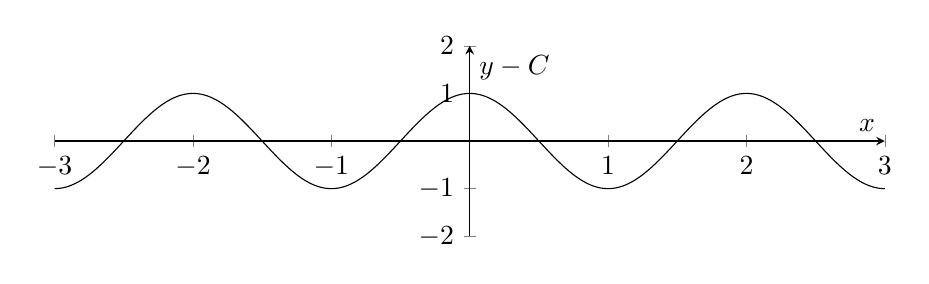
\begin{tikzpicture}
            \begin{axis}[
              axis lines=middle,
              xlabel=$x$,
              ylabel=$y - C$,
                xmin=-3, xmax=3,
                ymin=-2, ymax=2,
                width=\textwidth,
                height=4cm
            ]
              \addplot [domain=-3:3,samples = 1000] {1 * cos(deg(pi * x))};
            \end{axis}
          \end{tikzpicture}
    \end{center}

    当$t = 0.5$时,此时振幅为$\cos(0.5 \pi^2)$,$x = 0$为$\cos(0.5 \pi^2) + C$
    \begin{center}
        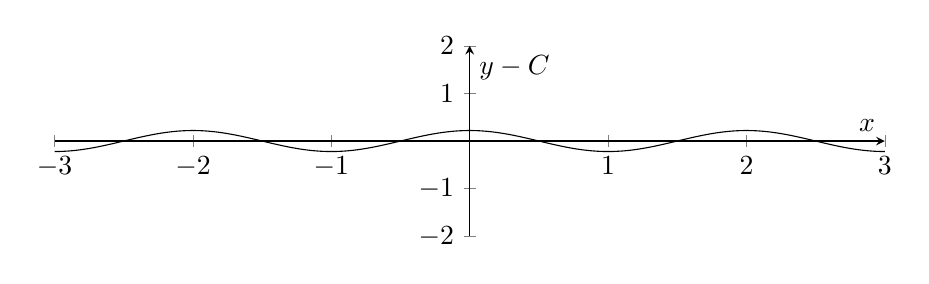
\begin{tikzpicture}
            \begin{axis}[
              axis lines=middle,
              xlabel=$x$,
              ylabel=$y - C$,
                xmin=-3, xmax=3,
                ymin=-2, ymax=2,
                width=\textwidth,
                height=4cm
            ]
              \addplot [domain=-3:3,samples = 1000] {cos(deg(0.5 * pi * pi)) * cos(deg(pi * x))};
            \end{axis}
          \end{tikzpicture}
    \end{center}

    当$t = 1$时,此时振幅为$-\cos(\pi^2)$,$x = 0$为$\cos(\pi^2) + C$
    \begin{center}
        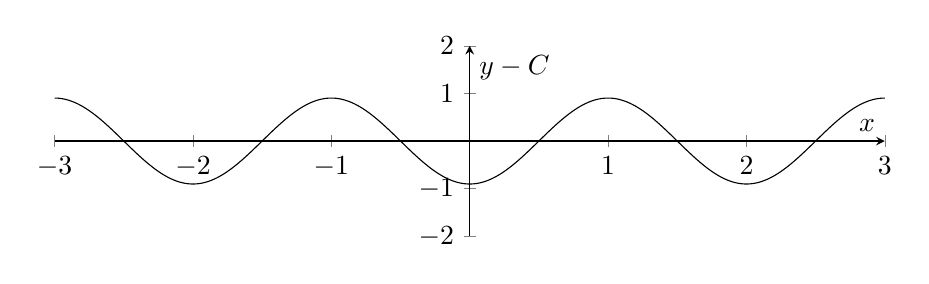
\begin{tikzpicture}
            \begin{axis}[
              axis lines=middle,
              xlabel=$x$,
              ylabel=$y - C$,
                xmin=-3, xmax=3,
                ymin=-2, ymax=2,
                width=\textwidth,
                height=4cm
            ]
              \addplot [domain=-3:3,samples = 1000] {cos(deg(1 * pi * pi)) * cos(deg(pi * x))};
            \end{axis}
          \end{tikzpicture}
    \end{center}

    当$t = 2$时,此时振幅为$\cos(2\pi^2)$,$x = 0$为$\cos(2\pi^2) + C$
    \begin{center}
        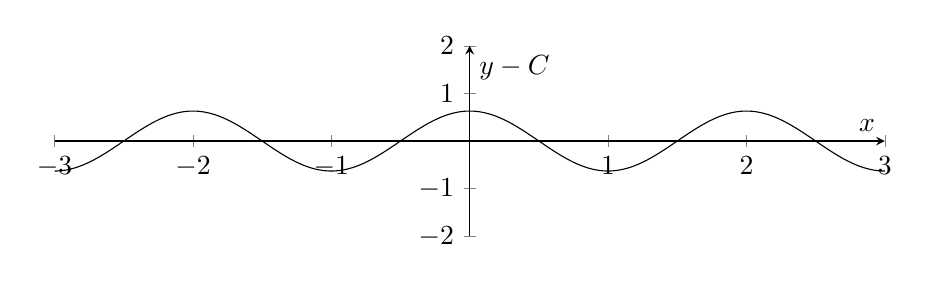
\begin{tikzpicture}
            \begin{axis}[
              axis lines=middle,
              xlabel=$x$,
              ylabel=$y - C$,
                xmin=-3, xmax=3,
                ymin=-2, ymax=2,
                width=\textwidth,
                height=4cm
            ]
              \addplot [domain=-3:3,samples = 1000] {cos(deg(2 * pi * pi)) * cos(deg(pi * x))};
            \end{axis}
          \end{tikzpicture}
    \end{center}

\end{exercise}

\begin{exercise}{16}
    \[u'_r = \frac{\partial u}{\partial x}\frac{\partial x}{\partial r} + \frac{\partial u}{\partial y}\frac{\partial y}{\partial r} + \frac{\partial u}{\partial z}\frac{\partial z}{\partial r} = u'_x \cos \varphi \cos \theta + u'_y \sin \varphi \cos \theta + u'_z \sin \theta\]

    \[u'_\varphi = \frac{\partial u}{\partial x}\frac{\partial x}{\partial \varphi} + \frac{\partial u}{\partial y}\frac{\partial y}{\partial \varphi} + \frac{\partial u}{\partial z}\frac{\partial z}{\partial \varphi} = - u'_x r \sin \varphi \cos \theta + u'_y r \cos \varphi \sin \theta \]

    \[u'_\theta = \frac{\partial u}{\partial x}\frac{\partial x}{\partial \theta} + \frac{\partial u}{\partial y}\frac{\partial y}{\partial \theta} + \frac{\partial u}{\partial z}\frac{\partial z}{\partial \theta} = - u'_x r \cos \varphi \sin \theta - u'_y r \sin \varphi \sin \theta + u'_z r \cos \theta\]

    由于二阶导数部分的项数过多,我们采用矩阵形式表示,
    \[u'_{rr} = \begin{pmatrix}
        \frac{\partial x}{\partial r}&\frac{\partial y}{\partial r}&\frac{\partial z}{\partial r}\\ 
    \end{pmatrix}
    \begin{pmatrix}
        u'_{xx}&u'_{xy}&u'_{xz}\\
        u'_{yx}&u'_{yy}&u'_{yz}\\
        u'_{zx}&u'_{zy}&u'_{zz}\\
    \end{pmatrix}
    \begin{pmatrix}
        \frac{\partial x}{\partial r}\\\frac{\partial y}{\partial r}\\\frac{\partial z}{\partial r}\\ 
    \end{pmatrix}
    +
    \begin{pmatrix}
        u'_x&u'_y&u'_z\\
    \end{pmatrix}
    \begin{pmatrix}
        \frac{\partial^2 x}{\partial r^2}\\\frac{\partial^2 y}{\partial r^2}\\\frac{\partial^2 z}{\partial r^2}\\        
    \end{pmatrix}
    \]

    \[u'_{r\varphi} = \begin{pmatrix}
        \frac{\partial x}{\partial r}&\frac{\partial y}{\partial r}&\frac{\partial z}{\partial r}\\ 
    \end{pmatrix}
    \begin{pmatrix}
        u'_{xx}&u'_{xy}&u'_{xz}\\
        u'_{yx}&u'_{yy}&u'_{yz}\\
        u'_{zx}&u'_{zy}&u'_{zz}\\
    \end{pmatrix}
    \begin{pmatrix}
        \frac{\partial x}{\partial \varphi}\\\frac{\partial y}{\partial \varphi}\\\frac{\partial z}{\partial \varphi}\\ 
    \end{pmatrix}
    +
    \begin{pmatrix}
        u'_x&u'_y&u'_z\\
    \end{pmatrix}
    \begin{pmatrix}
        \frac{\partial^2 x}{\partial r \partial \varphi}\\\frac{\partial^2 y}{\partial r \partial \varphi}\\\frac{\partial^2 z}{\partial r \partial \varphi}\\        
    \end{pmatrix}
    \]
    
    \[u'_{\theta\theta} = \begin{pmatrix}
        \frac{\partial x}{\partial \theta}&\frac{\partial y}{\partial \theta}&\frac{\partial z}{\partial \theta}\\ 
    \end{pmatrix}
    \begin{pmatrix}
        u'_{xx}&u'_{xy}&u'_{xz}\\
        u'_{yx}&u'_{yy}&u'_{yz}\\
        u'_{zx}&u'_{zy}&u'_{zz}\\
    \end{pmatrix}
    \begin{pmatrix}
        \frac{\partial x}{\partial \theta}\\\frac{\partial y}{\partial \theta}\\\frac{\partial z}{\partial \theta}\\ 
    \end{pmatrix}
    +
    \begin{pmatrix}
        u'_x&u'_y&u'_z\\
    \end{pmatrix}
    \begin{pmatrix}
        \frac{\partial^2 x}{\partial \theta\partial \theta}\\\frac{\partial^2 y}{\partial \theta\partial \theta}\\\frac{\partial^2 z}{\partial \theta\partial \theta}\\        
    \end{pmatrix}
    \]

    将已知的偏导数的值代入
    \[u'_{rr} = \begin{pmatrix}
        \cos \varphi \cos \theta&\sin \varphi \cos \theta&\sin \theta\\ 
    \end{pmatrix}
    \begin{pmatrix}
        u'_{xx}&u'_{xy}&u'_{xz}\\
        u'_{yx}&u'_{yy}&u'_{yz}\\
        u'_{zx}&u'_{zy}&u'_{zz}\\
    \end{pmatrix}
    \begin{pmatrix}
        \cos \varphi \cos \theta\\\sin \varphi \cos \theta\\\sin \theta\\ 
    \end{pmatrix}
    \]

    \[
    \begin{aligned}  
    u'_{r\varphi} = \begin{pmatrix}
        \cos \varphi \cos \theta&\sin \varphi \cos \theta&\sin \theta\\ 
    \end{pmatrix}&
    \begin{pmatrix}
        u'_{xx}&u'_{xy}&u'_{xz}\\
        u'_{yx}&u'_{yy}&u'_{yz}\\
        u'_{zx}&u'_{zy}&u'_{zz}\\
    \end{pmatrix}
    \begin{pmatrix}
        -r \sin \varphi \cos \theta \\r \cos \varphi \sin \theta \\0\\ 
    \end{pmatrix}\\
    &+
    \begin{pmatrix}
        u'_x&u'_y&u'_z\\
    \end{pmatrix}
    \begin{pmatrix}
        -\sin \varphi \cos \theta\\\cos \varphi \cos \theta\\0\\      
    \end{pmatrix}
    \end{aligned}  
    \]
    
    \[\begin{aligned}    
    u'_{\theta\theta} = \begin{pmatrix}
        -r \cos \varphi \sin \theta&- r \sin \varphi \sin \theta &r \cos \theta\\ 
    \end{pmatrix}&
    \begin{pmatrix}
        u'_{xx}&u'_{xy}&u'_{xz}\\
        u'_{yx}&u'_{yy}&u'_{yz}\\
        u'_{zx}&u'_{zy}&u'_{zz}\\
    \end{pmatrix}
    \begin{pmatrix}
        -r \cos \varphi \sin \theta\\- r \sin \varphi \sin \theta \\r \cos \theta\\ 
    \end{pmatrix}\\
    &+
    \begin{pmatrix}
        u'_x&u'_y&u'_z\\
    \end{pmatrix}
    \begin{pmatrix}
        -r \cos \varphi \cos \theta\\- r \sin \varphi \cos \theta \\- r \sin \theta\\        
    \end{pmatrix}
    \end{aligned}
    \]
    % \[
    % \begin{aligned}
    %     u'_{rr} &= \parameter{u'_{xx} \frac{\partial x}{\partial r} + u'_{xy} \frac{\partial y}{\partial r} + u'_{xz} \frac{\partial z}{\partial r}} \frac{\partial x}{\partial r} + u'_x \frac{\partial^2 x}{\partial r^2}\\
    %     &+ \parameter{u'_{yx} \frac{\partial x}{\partial r} + u'_{yy} \frac{\partial y}{\partial r} + u'_{yz} \frac{\partial z}{\partial r}} \frac{\partial y}{\partial r} + u'_y \frac{\partial^2 y}{\partial r^2}\\
    %     &+ \parameter{u'_{zx} \frac{\partial x}{\partial r} + u'_{zy} \frac{\partial y}{\partial r} + u'_{zz} \frac{\partial z}{\partial r}} \frac{\partial x}{\partial r} + u'_z \frac{\partial^2 z}{\partial r^2}\\
    %     &= 
    % \end{aligned}    
    % \]
\end{exercise}

\begin{exercise}{17}
    (1)
    首先我们先来导出$e^{x^2}$的$n$阶导数公式,这里我们利用了$Faà~di~Bruno's~formula$,可以证明有
    \[P_n(x) = \frac{n!}{(2x)^n} \sum_{k = \bracket{\frac{n+1}{2}}}^{n}C_{n}^{n - k} x^{2k}\]

    从而我们可以有$(e^{x^2})^{(n)} = \frac{n!}{(2x)^n} \sum_{k = \bracket{\frac{n+1}{2}}}^{n}C_{n}^{n - k} x^{2k} e^{x^2}$
    由于该函数是任意阶可微的,故任意阶偏导数都可以交换次序,因此我们不妨设对$x$求了$p \geq 0$阶偏导,对$y$求了$n - p$阶偏导,那么我们的结果有
    
    \[\frac{\partial^n f}{\partial x^p \partial y^{n - p}} = \frac{p!}{(2x)^p} \sum_{k = \bracket{\frac{p+1}{2}}}^{p}C_{p}^{p - k} x^{2k} e^{x^2 + y}\]

    从而我们可以得到泰勒公式[记$x - x_0 = h,y - y_0 = k$]
    \[f(x,y) = f(x_0,y_0) + \sum_{j = 1}^{n} \frac{1}{j !}\sum_{p = 0}^{n} C_{n}^{p} \frac{p!}{(2x)^p} \sum_{k = \bracket{\frac{p+1}{2}}}^{p}C_{p}^{p - k} x^{2k} e^{x^2 + y} h^p k^{n - p}\]

    (2)由于该函数是任意阶可微的,故任意阶偏导数都可以交换次序,因此我们不妨设对$x$求了$p \geq 0$阶偏导,对$y$求了$n - p$阶偏导,那么我们的结果有
    \[\frac{\partial^n f}{\partial x^p \partial y^{n - p}} = 2^{n - p} \sin(x + 2y + \frac{n\pi}{2})\]

    我们可以将泰勒公式写作以下形式[记$x - x_0 = h,y - y_0 = k$]
    \[f(x,y) = f(x_0,y_0) + \sum_{j = 1}^{n}\frac{1}{j !} \sum_{p = 0}^n C_{n}^p 2^{n - p} \sin(x + 2y +  \frac{n\pi}{2})h^p k^{n - p} + o(\Delta x^n)\]

    % (3)注意到
    % \[\frac{\partial f}{\partial x} = \lim_{x \to 0} \frac{\arctan(x^2 + 0) - \arctan(0)}{x} = \frac{2x}{1 + x^4}\]

    % 这个式子与$y$无关,利用对称性,我们知道$f$在$(0,0)$处的任何混合偏导数均为零,上式我们可以继续分解,如果利用复数的话,我们记
    % \[w_1 = \frac{\sqrt{2}}{2} + \frac{\sqrt{2}}{2} i,w_2 = -\frac{\sqrt{2}}{2} + \frac{\sqrt{2}}{2} i,w_3 = -\frac{\sqrt{2}}{2} - \frac{\sqrt{2}}{2} i,w_4 = \frac{\sqrt{2}}{2} - \frac{\sqrt{2}}{2} i\]

    % 即有
    % \[
    % \begin{aligned}
    %     \frac{2x}{1 + x4} &= \frac{1}{\sqrt{2}}\parameter{\frac{1}{x^2 - \sqrt{2} x + 1} + \frac{1}{x^2 + \sqrt{2} x + 1}}\\
    %     &= i \bracket{\frac{1}{x - w_2} + \frac{1}{x - w_4} - \frac{1}{x - w_1} - \frac{1}{x - w_3}}
    % \end{aligned}    
    % \]

    % 这样我们就把导数的形式变成了简单的形式,从而就有
    % \[\frac{\partial^n f}{\partial x^p \partial y^{n - p}} = \begin{cases}
    %     0, p \neq 0 ~and~ p \neq n\\
    %     i(-1)^{n - 1} (n - 1)! \bracket{\frac{1}{(x - w_2)^{n}} + \frac{1}{(x - w_4)^n} - \frac{1}{(x - w_1)^n} - \frac{1}{(x - w_3)^n}}, p = n\\
    %     i(-1)^{n - 1} (n - 1)! \bracket{\frac{1}{(y - w_2)^n} + \frac{1}{(y - w_4)^n} - \frac{1}{(y - w_1)^n} - \frac{1}{(y - w_3)^n}}, p = 0\\
    % \end{cases}\]

    % (这里我们可以将上面的复数全部化为实数的形式,但需要分奇偶讨论)因而我们的泰勒公式可以写作[记$x - 0 = h,y - 0 = k$]

    % \[f(x,y) = f(0,0) + \sum_{j = 1}^{n} \frac{1}{j !} \parameter{\frac{\partial^j f}{\partial x^j} h^j+ \frac{\partial^j f}{\partial y^j} k^j} + o(\Delta x^n)\]

    % (这里的两个$n$阶偏导数公式较长没有代入)

    (3)展开成为无穷级数讨论[先处理$\frac{1}{t^2 + 1}$,之后再考虑$\arctan t$]
\end{exercise}


\begin{exercise}{18}
    用极坐标的关系可以得到
    \[\begin{cases}
        \theta = \arctan \frac{y}{x}\\
        r = \sqrt{x^2 + y^2}\\
    \end{cases}\]   

    可以得到
    \[\frac{\partial \theta}{\partial x} = \frac{-y}{x^2 + y^2},\frac{\partial \theta}{\partial y} = \frac{x}{x^2 + y^2},\frac{\partial r}{\partial x} = \frac{x}{\sqrt{x^2 + y^2}},\frac{\partial r}{\partial y} = \frac{y}{\sqrt{x^2 + y^2}}\]

    利用链式法则有
    \[f_x = \frac{\partial f}{\partial \theta} \frac{\partial \theta}{\partial x} + \frac{\partial f}{\partial r} \frac{\partial r}{\partial x} = \frac{\partial f}{\partial \theta} \frac{-y}{x^2 + y^2} +  \frac{\partial f}{\partial r} \frac{x}{\sqrt{x^2 + y^2}}\]
    \[f_y = \frac{\partial f}{\partial \theta} \frac{\partial \theta}{\partial y} + \frac{\partial f}{\partial r} \frac{\partial r}{\partial y} = \frac{\partial f}{\partial \theta} \frac{x}{x^2 + y^2} +  \frac{\partial f}{\partial r} \frac{y}{\sqrt{x^2 + y^2}}\]

    代入我们条件的式子可以得到
    \[\sqrt{x^2 + y^2} \frac{\partial f}{\partial r} = 0\]

    如果我们考虑原点以外的点,那么就有
    \[\frac{\partial f}{\partial r} = 0\]

    故对于任何一个给定的$\theta_0$,$\varphi(r) = f(\theta_0,r)$的导数为零,利用一元微积分中的有限增量公式可知此函数为常数,因此$f$在极坐标下只是$\theta$的函数.
\end{exercise}


\begin{exercise}{19}
    (1)
    % 这个式子可以先化简,考虑对后面两项和差化积
    % \[\sin(x - y + z) + \sin(-x + y + z) = 2 \sin z \cos(x - y)\]

    % 这个方程实际上有闭合的解即

    对式子两侧微分可以得到
    \[
    \begin{aligned}
        &[\cos(x + y - z) - \cos(x - y + z) - \cos(-x + y + z)]dz \\
        =&[\cos(x + y - z) + \cos(x - y + z) - \cos(-x + y + z)]dx\\
        + &[\cos(x + y - z) - \cos(x - y + z) + \cos(-x + y + z)]dy
    \end{aligned}
    \]

    从而我们得到
    \[\frac{\partial z}{\partial x} = \frac{\cos(x + y - z) + \cos(x - y + z) - \cos(-x + y + z)}{\cos(x + y - z) - \cos(x - y + z) - \cos(-x + y + z)}\]
    \[\frac{\partial z}{\partial y} = \frac{\cos(x + y - z) - \cos(x - y + z) + \cos(-x + y + z)}{\cos(x + y - z) - \cos(x - y + z) - \cos(-x + y + z)}\]

    在一阶微分式的基础上再次进行微分,可以得到
    \[
        \begin{aligned}
            F\cdot (dz)^2+[\cos(x + y - z) - \cos(x - y + z) - \cos(-x + y + z)]d^2 z = - F\cdot(dx)^2 - F\cdot (dy)^2\\
        \end{aligned}
    \]

    由于$F(x,y,z) = 0$,故$d^2 z = 0$,那么也就有
    \[\frac{\partial^2 z}{\partial x^2} = \frac{\partial^2 z}{\partial y^2} = \frac{\partial^2 z}{\partial y \partial x} = \frac{\partial^2 z}{\partial x \partial y} = 0\]
        
    (2)我们对方程两侧微分

    \[\frac{dx}{\cos^2(x - z)} + \frac{dy}{\cos^2(y - z)} = \parameter{ \frac{1}{\cos^2(x - z)} + \frac{1}{\cos^2(y - z)} - e^z} dz\]

    从而有
    \[\frac{\partial z}{\partial x} = \frac{-\cos^2(y - z)}{\cos^2(x - z)\cos^2(y - z)e^z -\cos^2(y - z) - \cos^2(x - z)}\]
    \[\frac{\partial z}{\partial y} = \frac{-\cos^2(x - z)}{\cos^2(x - z)\cos^2(y - z)e^z -\cos^2(y - z) - \cos^2(x - z)}\]

    在一阶微分式的基础上继续微分,即可有
    \[
    \begin{aligned}
        &\bracket{e^z + \frac{2\tan(x - z)}{2\cos^2(x - z)} + \frac{\tan(y - z)}{\cos^2(y - z)}}(dz)^2-2\bracket{\frac{\tan(x - z)(dx)^2}{\cos^2(x - z)} + \frac{\tan(y - z)(dy)^2}{\cos^2(y - z)}} \\
        &= \parameter{ \frac{1}{\cos^2(x - z)} + \frac{1}{\cos^2(y - z)} - e^z} d^2 z\\
    \end{aligned}    
    \]
    由于各类三角函数写起来较为麻烦,我们这里记$\cos(x - z) := c_x,\cos(y - z) := c_y$,$\tan(x - z) := t_x,\tan(y - z) := t_y$

    那么有
    \[\frac{\partial^2 z}{\partial x^2} = \frac{e^z c_y^2 c_x^2 + 2t_x c_y^2 + 2t_x c_y^2}{(c_x^2 c_y^2 e^z - c_x^2 - c_y^2)^3}c_y^4 - \frac{2t_x c_y^2}{c_x^2 c_y^2 e^z - c_x^2 - c_y^2}\]
    \[\frac{\partial^2 z}{\partial y^2} = \frac{e^z c_y^2 c_x^2 + 2t_x c_y^2 + 2t_x c_y^2}{(c_x^2 c_y^2 e^z - c_x^2 - c_y^2)^3}c_x^4 - \frac{2t_y c_x^2}{c_x^2 c_y^2 e^z - c_x^2 - c_y^2}\]
    \[\frac{\partial^2 z}{\partial y\partial x} = \frac{\partial^2 z}{\partial x\partial y} = \frac{e^z c_y^2 c_x^2 + 2t_x c_y^2 + 2t_x c_y^2}{(c_x^2 c_y^2 e^z - c_x^2 - c_y^2)^3}c_x^2 c_y^2\]
    
    (3)我们对方程两侧进行微分
    \[xdx + y dy + zdz - \frac{dx}{\sqrt{x^2 - 1}} = 0\]

    我们可以得到
    \[\frac{\partial z}{\partial x} = \frac{1}{\sqrt{x^2 - 1}} - x, \frac{\partial z}{\partial y} = -y\]

    我们在前面的一阶微分式的基础上再次进行微分,可以得到
    \[(dx)^2 + (dy)^2 + (dz)^2 + z d^2 z = -\frac{x}{(x^2 - 1)^{\frac{3}{2}}}(dx)^2\]

    我们将前面求得的$dz$代入,即可得到各二阶偏导数
    \[\frac{\partial^2 z}{\partial x^2} = - \frac{1}{z} \bracket{1 + \frac{x}{(x^2 - 1)^{\frac{3}{2}}} + \frac{1}{z^2}\parameter{\frac{1}{\sqrt{x^2 - 1}} - x}^2}\]
    \[\frac{\partial^2 z}{\partial y^2} = - \frac{1}{z} \bracket{1 + \frac{y^2}{z^2}}\]
    \[\frac{\partial^2 z}{\partial y \partial x} = \frac{\partial^2 z}{\partial x \partial y} = - \frac{1}{z} \bracket{\frac{y}{z^2}\parameter{\frac{1}{\sqrt{x^2 - 1}} - x}}\]
\end{exercise}




\begin{exercise}{20}
    (1)根据上课时所讲的方法,我们对两个方程两侧进行微分,可以得到
    \[\begin{cases}
        du + 2 dv + 3 dx + 4 dy + 5 dz = 0\\
        du + 2v dv + 3x^2 dx + 4y^3 dy + 5z^4 dz = 0\\
    \end{cases}\]
    可以解得
    \[du = \frac{3v - 3 x^2}{v - 1} + \frac{4 v - 4 y^3}{v - 1}dy + \frac{5v - 5z^4}{v - 1}dz\]

    由于我们的两个方程对应的函数显然是连续可微的,因而有
    \[\frac{\partial u}{\partial x} = \frac{3v - 3x^2}{v - 1}\]

    我们在之前第一次微分得到的式子的基础上再做一次微分,注意此时$x,y,z$是自变量,因此
    \[\begin{cases}
        d^2 u + 2 d^2 v = 0\\
        d^2 u + 2 (dv)^2 + 2 v d^2 v + 6x (dx)^2 + 12 y^2 (dy)^2 + 20 z^3 (dz)^2 = 0\\
    \end{cases}\]

    消元并移项得到
    \[d^2 u = -\frac{2}{1 - v}(dv)^2 - \frac{6x}{1 - v}(dx)^2 -\frac{12y^2}{1 - v}(dy)^2 - \frac{20}{1 - v}z^3(dz)^2 \]

    其中的$dv$我们利用第一次的微分式可以得到
    \[dv = -\frac{3x^2 - 3}{2v - 2}dx - \frac{4y^3 - 4}{2v - 2} dy - \frac{5z^4 - 5}{2v - 2}dz\]

    由于全部展开项数比较多,我们只保留我们要求的项,可以求得
    \[\frac{\partial^2 u}{\partial x^2} = \frac{6x}{v - 1} + \frac{2}{v - 1}\parameter{\frac{3x^2 - 3}{2v - 2}}^2 = \frac{6x}{v - 1} + \frac{9(x^2 - 1)^2}{2(v - 1)^3} \]
    \[\dfrac{\partial^2 u}{\partial x \partial y} = \frac{2}{v - 1} \cdot \frac{3x^2 - 3}{2v - 2} \frac{4y^3 - 4}{2v - 2} = \frac{6(x^2 - 1)(y^3 - 1)}{(v - 1)^3}\]
    
    (2)由于一阶微分的形式不变性,这里我们的
    \[\frac{\partial u}{\partial x} = \frac{3v - 3x^2}{v - 1}\]
    的结果保持不变

    但是二阶微分的处理发生了不同,注意我们这里以$x,y,v$为自变量,因而对一阶微分式子在此进行微分可以得到
    \[\begin{cases}
        d^2 u + 5 d^2 z = 0\\
        d^2 u + 2 (dv)^2 + 6x (dx)^2 + 12 y^2 (dy)^2 + 20 z^3 (dz)^2 + 5 z^4 d^2 z = 0\\
    \end{cases}\]

    消元移项可以得到
    \[d^2 u = \frac{2}{z^4 - 1}(dv)^2 + \frac{6x}{z^4 - 1}(dx)^2 + \frac{12y^2}{z^4 - 1}(dy)^2 + \frac{20z^3}{z^4 - 1}(dz)^2\]

    其中的$dz$可以利用前面的一阶微分式进行消元得到
    \[dz = -\frac{2v - 2}{5z^4 - 5}dv - \frac{3x^2 - 3}{5z^4 - 5}dx - \frac{4y^3 - 4}{5z^4 - 5}dy\]

    我们可以求得
    \[\frac{\partial^2 u}{\partial x^2} = \frac{6x}{z^4 - 1} + \frac{20z^3}{z^4 - 1}\parameter{\frac{3x^2 - 3}{5z^4 - 5}}^2 = \frac{6x}{z^4 - 1} + \frac{36(x^2 - 1)^2 z^3}{5(z^4 - 1)^3}\]
    \[\frac{\partial^2 u}{\partial x \partial y} = \frac{20z^3}{z^4 - 1}\cdot \frac{3x^2 - 3}{5z^4 - 5} \frac{4y^3 - 4}{5z^4 - 5} = \frac{48(x^2 - 1)(y^3 - 1)z^3}{5(z^4 - 1)^3}\]
\end{exercise}

\end{CJK}
\end{document}

\begin{itemize} 
\end{itemize}